\chapter{Implementacja sterowania NAO}
\label{chap:implementacja}

W rozdziale opisano środowisko służące do testowania i demonstracji omawianej technologii. W tym celu sformułowano proste zadanie, dla którego zaproponowano dwa rozwiązania. Pierwsze opiera się na automacie skończonym (zaimplementowanym z użyciem biblioteki SMACH),
%pozwoliło na realizację zadania. 
drugie, korzysta z systemu planowania zadań (bazujące na implementacji RGOAP).%, mimo braku zgłoszenia błędu nie pozwoliło na realizację zadania.
Powyższe rozwiązania ukazują od strony technicznej zagadnienia poruszane we wcześniejszych rozdziałach.

\section{Środowisko programowe}
\label{sec:srodowisko}

Aby dokonać testów sterowania robotem NAO konieczne było zbudowanie środowiska integrującego potrzebne w tej pracy oprogramowanie. Poniżej opisano elementy wchodzące w jego skład. 

\begin{description}
\item[Ubuntu 14.04.1 Trusty Tahr] {System operacyjny, wywodząca się z Debiana dystrybucja \textit{GNU/Linux} o statusie LTS (long term support – ang. długi okres wsparcia).~\cite{UBUN} % Ze względu na dużą społeczność użytkowników posiada bogate repozytoria i jest wspierana przez producentów oprogramowania. Została wybrana wersja \textit{14.04.01}, ponieważ używany ROS Indigo jest przeznaczony natywnie na to wydanie Ubuntu. W przypadku wyboru nowszej wersji, np. \textit{Ubuntu 14.04.5} przed instalacją ROS konieczne jest wykonanie wszystkich zalecanych aktualizacji systemu w celu naprawienia uszkodzonych zależności systemowych.
System został zainstalowany z jądrem \textit{GNU/Linux} w wersji \textit{3.13.0-161-generic} i posiada kompilator \textit{gcc} w wersji \textit{Ubuntu 4.8.4-2ubuntu1~14.04.4}.}

\item[Python 2.7.6] {Skryptowy, zorientowany obiektowo język programowania.~\cite{PYTH2} Jest obecnie wydawany w wersjach 2.x oraz 3.x.}

\item[ROS Indigo Igloo] {Oprogramowanie ułatwiające sterowanie robotami, robotyczny system operacyjny.~\cite{ROS} % Zapewnia zbiór narzędzi umożliwiających nadawanie i odbieranie wiadomości, tworzenie symulacji. Standaryzuje komunikację między elementami architektury sterowania zapewniając szkielet wiadomości (ang. messages), nadawców (ang. publisher) i serwisów (ang. services). zewnętrzne biblioteki, integracja z Pythonem, C++, przeglądarkami internetowymi.

Wersja Indigo wspiera dodawanie pakietów z użyciem systemu \textit{rosbuild}, co było istotne w początkowych fazach implementacji środowiska RGOAP. Wykorzystano następujące narzędzia:
\begin{description}
\item[rospy] {Python został wykorzystany w ROS, aby umożliwić programistom szybkie prototypowanie i implementację rozwiązań w zastosowaniach niewymagających wysokiej wydajności.~\cite{ROSPY} ROS korzysta z wersji 2.x, w celu zachowania zgodności wstecznej.}
\item[NAO] {ROS udostępnia pakiety \textit{nao\_robot} (zawierający w szczególności \textit{nao\_bringup}) oraz \textit{nao\_extras} umożliwiające sterowanie robotem NAO.~\cite{ROSnao}}
\item[SMACH] {Biblioteka napisana w Pythonie służąca do tworzenia automatów skończonych. Została stworzona przez deweloperów ROSa i domyślnie jest instalowana razem z nim, ale jest projektem niezależnym i może być używana osobno. Integrację z ROSem zapewnia pakiet \textit{smach\_ros}. Przydatny jest również \textit{smach\_viever} tworzący graf obrazujący stany automatu w czasie rzeczywistym. Biblioteka ta jest wykorzystywana w zastosowaniach robotycznych.~\cite{FOUK}}

\item[RGOAP] {Robotyczna implementacja architektury GOAP autorstwa Felixa Kolbe będąca przedmiotem pracy magisterskiej~\cite{KOLB}.  

Metapakiet \textit{executive\_rgoap}~\cite{EXECrgoap} zawiera trzy pakiety: \textit{rgoap}, \textit{rgoap\_ros}, \textit{rgoap\_smach}. Pierwszy, \textit{rgoap}, zapewnia podstawową implementację środowiska GOAP. Jest niezależną od ROSa biblioteką napisaną w Pythonie, która jednak sama w sobie jest niekompletna. Przy wykorzystywaniu jej konieczne jest tworzenie klas pochodnych z przeciążaniem metod. Pakiet \textit{rgoap\_ros} przeciąża wybrane klasy czym zapewnia komunikację z ROSem inicjalizując odpowiednie wątki (ang. \textit{nodes}). Pakiet \textit{rgoap\_smach} wykorzystuje bibliotekę SMACH, co umożliwia generowanie (i analizę wygenerowanych) automatów skończonych w czasie rzeczywistym. 
RGOAP umożliwia również wykorzystanie jako akcji automatów SMACH stworzonych niezależnie od RGOAP.

RGOAP powstało w 2013 roku, na wersję ROS Groovy,\cite{EXECrgoap} którego kod źródłowy jest dostępny w repozytorium~\cite{KOLBrgoap}. Do budowy pakietu należy wykorzystać narzędzie rosbuild. W celu zapewnienia większej przenośności przebudowano strukturę plików pakietu, catkinizując RGOAP. Efekt pracy można pobrać z repozytorium~\cite{TARNrgoap}.

}
\end{description}
\item[NAOqi 2.1.2] {System operacyjny oparty o jądro Linux autorstwa firmy Aldebaran, pozwalający na sterowanie robotem NAO, programowanie go oraz utworzenie wirtualnego agenta podłączonego do symulacji.~\cite{NAOqi} Instancja NAOqi działa na komputerze pokładowym robota. Producent dostarcza zestaw narzędzi, pozwalających na pisanie programów w językach C++, Java lub Python. NAOqi może zostać uruchomione niezależnie od innych aplikacji z poziomu terminala. Wymagana jest wersja \textit{2.1.2}, w celu zachowania kompatybilności z ROSem.~\cite{ROSnaoinstall}}

\item[Choreographe 2.1.2] {Aplikacja okienkowa, umożliwiająca tworzenie scenariuszy działania robota w formie graficznej. Choreographe dostarcza bibliotekę akcji w postaci bloków, możliwych do połączenia przez programistę w automat skończony. Dzięki aplikacji można w łatwy sposób podłączyć się do fizycznego robota, utworzyć symulację, bądź połączyć się z działającą w systemie instancją NAOqi. W jednej z zakładek można zobaczyć wizualizację stanu robota, która działa wydajniej, niż inne dostępne rozwiązania. Jak w przypadku NAOqi wymagana jest wersja \textit{2.1.2}.~\cite{ROSnaoinstall}}
}
\end{description}



\section{Studium przypadku: ,,Ćwiczenia gimnastyczne''}
\label{sec:koncepcja}
Scenariusz studium przypadku jest następujący. Robot NAO ma wykonać trzy przysiady. Po wykonaniu ćwiczenia robot siada. W trakcie trwania zadania NAO powinien siedmiokrotnie zmienić swoją pozę. 

Poniżej zaproponowano i omówiono dwa rozwiązania problemu. Pierwsze wykorzystuje automat skończonym drugie jest oparte o system planowania działań. Niezależnie od rozwiązania wykorzystywany jest identyczny interfejs robota przygotowany w oddzielnej klasie.

\subsection{Automat skończony}
\label{subsec:k_automat}
Z wykorzystaniem automatu skończonego zadanie można sprowadzić do zdefiniowania trzech stanów. Przy aktywacji stanu robot przyjmuje ustaloną pozę. Warunki opisujące przejścia między stanami są zdefiniowane wewnątrz automatu z użyciem prostej pętli. 

Korzystając z biblioteki SMACH napisano skrypt, który pozytywnie realizuje postawione zadanie.

\subsection{System planowania działań}
\label{subsec:k_goap}
Rozwiązanie korzystające z systemu planowania działań zostało podzielone na dwa podzadania. Pierwsze sprowadzało się do opisania agenta, czyli jego stanu wiedzy, dostępnych akcji i pożądanych celów. Drugie podzadanie polegało na użyciu narzędzi dostarczonych przez system.

%W implementacji wykorzystano środowisko RGOAP. Niestety nie uzyskano pozytywnego wyniku, pomimo opisania agenta zgodnie z dokumentacją i wyeliminowania wszystkich błędów zgłaszanych podczas debugowania skryptu.

\section{Implementacja}
\subsection{Klasa robot}
Aby móc testować robota zdefiniowano klasę \textit{Robot}. Została użyta w kolejnych skryptach, aby zapewnić jednolity interfejs i zwiększyć czytelność kodu. Przed jej użyciem należy włączyć fizycznego robota, lub uruchomić program Choreographe z symulacją.
Po zaimportowaniu biblioteki \textit{rospy} oraz klasy \textit{ALProxy} z biblioteki \textit{naoqi} możliwe jest połączenie się z robotem. Wymaga to użycia trzech linijek kodu: definiującej numery IP, numer portu oraz aktywującej kompetencje robota.

Domyślny port fizycznego robota to \textit{9559}. %, przy korzystaniu z symulacji należy podmienić numer.

\lstinputlisting[language=Python,linerange=7-11,firstnumber=7]{scripts/robot.py}

Funkcja aktywująca kompetencje została wydzielona, a jej kod jest załączony poniżej. Aktywowano w niej trzy moduły zarządzające kompetencjami. Pierwszy \textit{ALRobotPosture} pozwala na zdefiniowanie kilku ustalonych pozycji, drugi \textit{ALTextToSpeech} pozwala robotowi na wydawanie dźwięków, a trzeci \textit{ALMotion} pozwala na wydawanie poleceń takich jak obrót lub marsz. Pełna lista modułów znajduje się na stronie \cite{NAOqimodules}. 
\lstinputlisting[language=Python,linerange=14-17,firstnumber=14]{scripts/robot.py}

W klasie robota zdefiniowano kilka metod realizujących ruch. 
%To jedynie nakładki na gotowe funkcje, a ich szablon wykorzystuje schemat kodu generowanego automatycznie w bloczkach programu Choreographe. 
Przed wykonaniem akcji sprawdzane jest połączenie z robotem, a po jej wykonaniu sprawdzana jest poprawność zwróconego przez nią wyjścia. Pozwala to na przerwanie programu w przypadku niepowodzenia, lub wywołanie innych funkcji, mających przywrócić pożądany stan. 

\lstinputlisting[language=Python,linerange=19-25,firstnumber=19]{scripts/robot.py}

Implementacja klasy robota jest bardzo prosta, ponieważ zaproponowany problem nie wymaga niczego więcej. W bardziej skomplikowanych przypadkach można umieścić w klasie prosty automat skończony oparty o konwencję opisaną w rozdziale \ref{subsec:3stany}. Jak wspomniano w rozdziale \ref{subsec:GOAP_CERT} poza wymienionymi trzema stanami można dodać kolejne narzędzia, uwzględniające problemy robotów, z jakimi nie spotykają się bohaterowie niezależni. Dla przykładu robot może posiadać dodatkowy stan zmieniający jego zachowanie w przypadku usterki, upadku lub niskiego napięcia w bateriach. 

\subsection{SMACH}
\label{subsec:i_automat}
Poniżej omówiono implementację rozwiązania sformułowanego w rozdziale~\ref{subsec:k_automat}. 

Skrypt jest przygotowany do wywołania go w terminalu. Przed uruchomieniem należy nadać mu właściwe uprawnienia wykonalności. 
\lstinputlisting[language=Python,linerange=1-1,firstnumber=1]{scripts/smach_runner.py}

Do skryptu zaimportowano trzy biblioteki: \textit{rospy} umożliwiającą na komunikację z ROSem, \textit{smach} udostępniającą klasy pozwalające na definiowanie stanów i całego automatu skończonego, oraz \textit{smach\_ros} zapewniającego komunikację między biblioteką a ROSem. Pakiet SMACH jest instalowany domyślnie z ROSem, więc z poziomu Pythona biblioteki są importowane bez żadnych dodatkowych działań. 
\lstinputlisting[language=Python,linerange=3-5,firstnumber=3]{scripts/smach_runner.py}

Z pliku \textit{robot.py} pobrano klasę \textit{Robot}, która została następnie użyta w funkcji \textit{main()} do utworzenia instancji robota. Poza tą linijką klasa nie jest używana jawnie – utworzony obiekt jest przekazywany jako argument 
\lstinputlisting[language=Python,linerange=7-7,firstnumber=7]{scripts/smach_runner.py}
\lstinputlisting[language=Python,linerange=44-45,firstnumber=44]{scripts/smach_runner.py}

Następnie zadeklarowano trzy klasy \textit{POSE\_ZERO}, \textit{POSE\_CROUCH} oraz \textit{SIT\_POSE}, dziedziczące po klasie \textit{smach.State}. Każda z klas reprezentuje inny stan automatu. Konieczne jest przeciążenie dwóch metod: konstruktora oraz \textit{execute()}.

Do konstruktorów zadeklarowanych stanów przekazano jako argument referencję na instancję robota. 
Wywoływany jest konstruktor klasy \textit{smach.State} który pozwala na określenie dostępnych wyjść stanu (\textit{outcomes}). W konstruktorze mogą zostać zdefiniowane zmienne opisujące stan wewnętrzny stanu. W przypadku klasy \textit{POSE\_ZERO} jest to licznik przysiadów (\textit{counter}).

Przy deklaracji stanu konieczne jest przeciążenie metody \textit{execute()}. Jest ona wykonywana przy każdej aktywacji stanu. Zgodnie z konwencją przyjmuje argument \textit{userdata}. Może zwracać jedynie określone w konstruktorze wyjścia. 

W przypadku \textit{POSE\_ZERO} przy aktywacji \textit{execute()} wyświetlana wiadomość o aktywacji stanu. Następnie robotowi wydawana jest komenda zmieniająca jego pozycję. Na końcu umieszczony jest warunek zwracający jedno z dwóch wyjść: \textit{outcome1}, gdy ćwiczenie (wystarczająca liczba przysiadów) nie zostało jeszcze wykonane oraz \textit{outcome2}, gdy robot ma zakończyć ćwiczenie i usiąść.

\lstinputlisting[language=Python,linerange=9-22,firstnumber=9]{scripts/smach_runner.py}

W funkcji \textit{main()} tworzona jest instancja automatu skończonego. Przypisywane są mu zdefiniowane wcześniej stany. Metoda \textit{add()} przyjmuje trzy argumenty: nazwę stanu, instancję stanu tworzoną przez wywołanie konstruktora, oraz informację o przejściach między stanami, gdy metoda \textit{execute()} zwróci określone z wyjść.

\lstinputlisting[language=Python,linerange=47-55,firstnumber=47]{scripts/smach_runner.py}

Po zdefiniowaniu automatu jest on aktywowany z wykorzystaniem metody \textit{execute()}. Oprócz tego uruchamiany jest tzw. introspektor, pozwalający na analizę automatu w czasie rzeczywistym z wykorzystaniem ROSa. Aby narzędzie do analizy nie wyłączało się zaraz po zakończeniu pracy automaty dodano linijkę zawieszającą skrypt.

\lstinputlisting[language=Python,linerange=57-63,firstnumber=57]{scripts/smach_runner.py}

Aby uruchomić skrypt należy:
\begin{itemize}
\setlength\itemsep{-0.5em}
    \item uruchomić lub zasymulować robota, a następnie zaktualizować port i adres IP w skrypcie \textit{robot.py};
    \item zainicjować w terminalu ROSa komendą: \textit{roscore};
    \item w drugim oknie terminala wywołać skrypt komendą: \textit{./smach\_runner.py};
    \item w trzecim oknie terminala uruchomić introspektor komendą: \textit{rosrun smach\_viever smach\_viever.py}.
\end{itemize}

Zadanie zrealizowane w ten sposób przez wirtualnego NAO zostało przedstawione na rysunku \ref{fig:NAOsmach}.

\begin{figure}
\centering
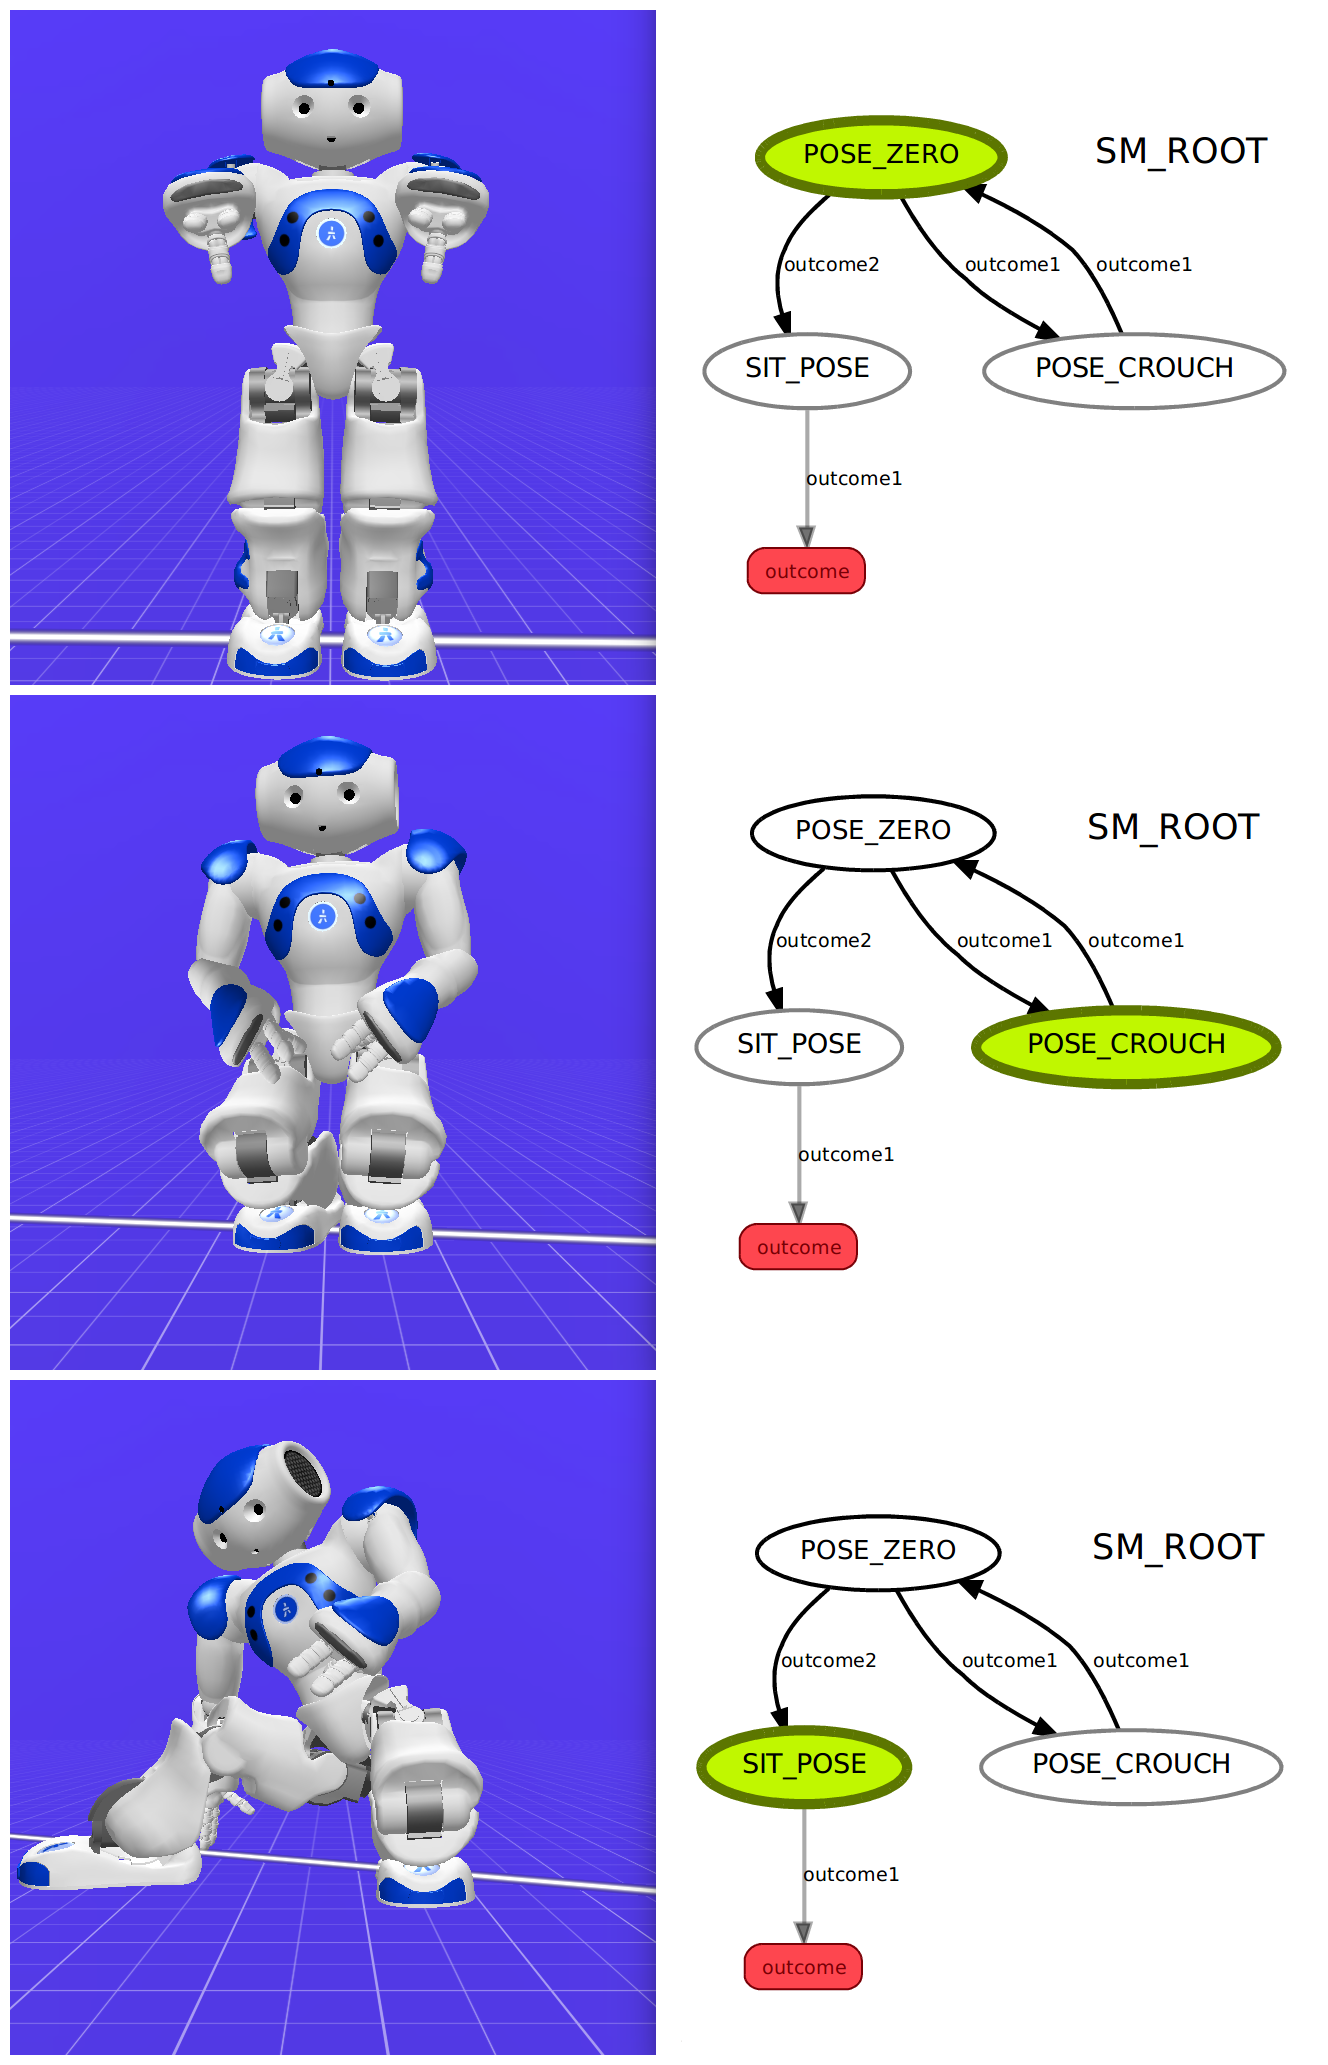
\includegraphics[width=0.90\textwidth]{images/NaoSmachPoses.png}
\caption{Wirtualny robot zwizualizowany w Choreographe sterowany przez automat skończony SMACH.}
\label{fig:NAOsmach}
\end{figure}

\subsection{RGOAP}
\label{subsec:i_goap}

Poniżej omówiono implementację rozwiązania sformułowanego w rozdziale~\ref{subsec:k_goap}, czyli zawartość skryptów \textit{rgoap\_agent.py} definiującego kompetencje agenta oraz \textit{rgoap\_runner.py} uruchamiającego narzędzia środowiska RGOAP. 

\subsubsection{Skrypt rgoap\_agent.py}
Podobnie jak w przypadku rozwiązania korzystającego z biblioteki SMACH w skrypcie opisującym agenta wykorzystano klasę \textit{Robot}. Utworzono globalną instancję NAO. Obiekt ten został użyty przy implementacji akcji opisanych kilka akapitów niżej.

\lstinputlisting[language=Python,linerange=3-4,firstnumber=3]{scripts/rgoap_agent.py}

Zaimportowano niezbędne narzędzia. Z biblioteki \textit{rgoap} pobrano klasy realizujące zadania elementów opisanych w rozdziale \ref{subsec:GOAP_elem}. Klasy \textit{Condition} i \textit{Action} nie są w pełni zaimplementowane, dlatego konieczne było użycie klas pochodnych z biblioteki \textit{rgoap\_ros} a więc \textit{ROSTopicCondition} oraz \textit{ROSTopicAction}. Pozwala to na wykorzystanie ROSa jako środowiska zarządzającego wiedzą robota. Ze zbioru standardowych wiadomości ROSa zaimportowano \textit{String}, który będzie typem danych przechowanych w stanach atomowych.

\lstinputlisting[language=Python,linerange=6-9,firstnumber=6]{scripts/rgoap_agent.py}

Zgodnie z ustaloną konwencją w zdefiniownano funkcję \textit{get\_all\_conditions()}. Funkcja zwraca listę stanów atomowych opisujących model świata agenta. Umieszczono w niej dwa stany: \textit{robot.pose} opisujący aktualną pozę robota oraz \textit{robot.squat} informującą, czy ćwiczenie gimnastyczne zostało już wykonane.

Z punktu widzenia modelu BDI to w tym miejscu mogą zostać zdefiniowane wiedza i przekonania agenta. 

Konstruktor klasy \textit{ROSTopicCondition} przyjmuje cztery argumenty: nazwę stanu, nazwę tematu, typ danych będący wiadomością zdefiniowaną w ROSie oraz pole typu danych.
Nazwa stanu jest jego identyfikatorem. Z poziomu skryptu nie jest konieczne używanie zmiennej do której stan został przypisany, ponieważ referencję na stan zwróci metoda \textit{Condition.get()}. Druga nazwa jest wykorzystana przez ROS do utworzenia odpowiedniego tematu (ang. topic). Temat będzie przechowywał wskazany typ danych i umożliwiał wysyłanie do niego wiadomości tego typu. W ROSie wiadomości składają się z wielu pól (ang. field), więc temu samemu tematowi może być przypisane wiele stanów atomowych (po jednym na każde pole).  
\lstinputlisting[language=Python,linerange=60-64,firstnumber=60]{scripts/rgoap_agent.py}

Zdefiniowano trzy akcje i podobnie jak w przypadku stanów zdefiniowano funkcję zwracającą ich listę. Dla każdej akcji utworzona została klasa dziedzicząca po \textit{ROSTopicAction}. Szczegóły implementacyjne są omawiane poniżej. 

Pierwsza z akcji \textit{ActionStandUp()} pozwala na ułożenie agenta w pozycji początkowej. Z poziomu modelu świata akcja umożliwia zmianę wartości stanu \textit{robot.pose} z \textit{init} na \textit{stand\_up}. 

Druga akcja \textit{ActionSquat()} umożliwia robotowi wykonanie trzech przysiadów. Aby akcja mogła zostać podjęta robot musi wstać. Innymi słowy warunkiem jest wcześniejsze ustalenie wartości stanu \textit{robot.pose} na \textit{stand\_up}. Efektem akcji jest realizacja ćwiczenia gimnastycznego, czyli zmiana wartości stanu \textit{robot.squat} na \textit{ready}. 

Warunkiem podjęcia trzeciej akcji \textit{ActionSit()} jest zrealizowanie ćwiczenia i wyprostowana poza. Podjęcie akcji spowoduje że robot usiądzie zmieniając wartość stanu \textit{robot.pose} na \textit{sit}. 

Powyższe akcje są bardzo proste, ponieważ służyły one do testowania środowiska. %, a nie do realnych problemów. 
Akcje mogą zostać złożone przez planer w sekwencje. W modelu BDI takie sekwencje można interpretować jako realizację intencji. Im więcej zdefiniowanych akcji, tym bardziej skomplikowane intencje mogą być realizowane przez agenta.
\lstinputlisting[language=Python,linerange=66-70,firstnumber=66]{scripts/rgoap_agent.py}

Jak wspomniano powyżej, do zdefiniowania akcji konieczne jest utworzenie klasy dziedziczącej po \textit{ROSTopicAction}. W takiej klasie należy napisać konstruktor i przeciążyć trzy metody: \textit{run()}, \textit{cost()} oraz \textit{check\_freeform\_conditions()}. 

W konstruktorze wykorzystywany jest konstruktor klasy nadrzędnej, który przyjmuje cztery argumenty: nazwę tematu ROS, który będzie powiązany z akcją, typ ROSowej wiadomości przekazywanej do tematu, oraz dwie listy zawierające warunki i efekty. 

W metodzie \textit{run()} określone są działania agenta wykonywane gdy akcja zostanie aktywowana. 

Metoda \textit{cost()} musi zwracać pewną liczbę, która zostanie użyta przez planner do określenia optymalnej sekwencji akcji. W tym przypadku koszt jest stały, ale nic nie stoi na przeszkodzie, żeby koszt wyliczać dynamicznie w zależności od stanu środowiska agenta.

Ostatnia metoda \textit{check\_freeform\_conditions()} musi zwracać wartość logiczną. Akcja zostanie wykonana, tylko jeśli zostanie zwrócona wartość \textit{True}. Pozwala to na określenie zewnętrznych warunków wykorzystania akcji.

Ponieważ wewnątrz \textit{cost()} oraz \textit{check\_freeform\_conditions()} możliwe jest umieszczenie skomplikowanych warunków, jest to kolejne po stanach świata miejsce, w którym agent BDI może przechowywać swoje przekonania.
\lstinputlisting[language=Python,linerange=11-22,firstnumber=11]{scripts/rgoap_agent.py}

Podobnie jak w przypadku stanów atomowych i akcji należy zdefiniować funkcję zwracającą listę wszystkich celów agenta. W omawianym zadaniu cel jest tylko jeden: \textit{GoalReady()}. Agent chce zakończyć ćwiczenie i usiąść. 

Cele są urzeczywistnionymi pragnieniami agenta BDI. Funkcja nie musi przechowywać statycznej listy celów. Może ona generować listę celów reagując na zmiany środowiska niezależne od stanu świata postrzeganego przez agenta. W szczególności na cele mogą wpływać polecenia od innych agentów.
\lstinputlisting[language=Python,linerange=72-73,firstnumber=72]{scripts/rgoap_agent.py}

Przy implementowaniu celów należy utworzyć klasę dziedziczącą po klasie \textit{Goal}, jednak nie ma potrzeby przeciążania żadnych metod. Wywoływany jest jedynie konstruktor klasy nadrzędnej z dwoma argumentami: listą warunków, które definiują cel oraz liczbą określającą atrakcyjność celu. Gdyby zdefiniowanych zostało wiele sprzecznych celów, do realizacji przekazany zostanie najatrakcyjniejszy, niewykluczający się zbiór.
\lstinputlisting[language=Python,linerange=53-58,firstnumber=53]{scripts/rgoap_agent.py}

Listy stanów, akcji oraz celów w pełny sposób opisują agenta. Tak przygotowany plik można wykorzystać w kolejnym skrypcie, zarządzającym pracą środowiska RGOAP.

\subsubsection{Skrypt rgoap\_runner.py}

Uruchamiając środowisko RGOAP należy zaimportować: skrypt ze wcześniej zdefiniowanym agentem, \textit{rospy}, czyli bibliotekę pozwalającą na obsługę ROSa, wszystkie rodzaje wiadomości, jakie zostały użyte przy tworzeniu tematów opisujących stany i akcje agenta (w tym przypadku tylko wiadomość \textit{String}), oraz klasy \textit{Runner} i \textit{Condition} z biblioteki \textit{rgoap}. 
\lstinputlisting[language=Python,linerange=3-10,firstnumber=3]{scripts/rgoap_runner.py}

W skrypcie zdefiniowano funkcję \textit{tasker()}, która zarządza całym środowiskiem. Inicjuje one węzeł (ang. node) ROSa, umożliwiając komunikację i przechowuje instancję nadzorcy (ang. runner), zarządzającego wszystkimi narzędziami środowiska RGOAP. Tworząc obiekt klasy \textit{Runner} jako argument należy przekazać zaimportowany moduł z definicją agenta. Nadzorca wykorzystuje funkcje \textit{get\_all\_conditions()} oraz \textit{get\_all\_actions()} do zainicjowania środowiska.
\lstinputlisting[language=Python,linerange=12-14,firstnumber=12]{scripts/rgoap_runner.py}

Przed uruchomieniem środowiska należy zadeklarować stan świata. Stanom atomowym przypisano tematy w ROSie, więc należy przekazać do nich wartość. W tym celu zdefiniowani zostali dwaj nadawcy (ang. publisher). Metodą \textit{publish()} wysyłane są odpowiednie wiadomości.
\lstinputlisting[language=Python,linerange=16-22,firstnumber=16]{scripts/rgoap_runner.py}

Po zadeklarowaniu stanu świata wywołuje się metodę \textit{plan\_and\_execute\_goals()} na obiekcie nadzorcy. Jako argument przekazywana jest lista celów do realizacji. 
\lstinputlisting[language=Python,linerange=24-26,firstnumber=24]{scripts/rgoap_runner.py}

Aby uruchomić skrypt należy podobnie jak w przypadku SMACH: 
\begin{itemize}
\setlength\itemsep{-0.3em}
\item uruchomić program Choreographe lub połączyć się z inną instancją robota NAO, wprowadzając właściwy adres IP oraz numer portu w skrypcie \textit{robot.py};
\item w terminalu utworzyć instancję systemu ROS wpisując komendę: \textit{roscore};
\item w drugim oknie terminala (aby biblioteki wykorzystane w skrypcie zostały zaimportowane) załadować wcześniej zbudowany pakiet RGOAP, np. z wykorzystaniem komendy: \textit{source ~/catkin\_rgoap/devel/source.bash};
\item w tymże oknie terminala uruchomić skrypt komendą: \textit{./rgoap\_runner.py}.
\end{itemize}

Niestety po uruchomieniu skryptu środowisko bez zgłaszania błędów, osiąga limit kroków planowania (ustawiony na 500) nie znajdując żadnego planu. Z powodu ubogiej dokumentacji i braku reakcji ze strony twórców oprogramowania na zapytania nie udało się rozwiązać tego problemu. 